\documentclass[conference]{IEEEtran}
\IEEEoverridecommandlockouts

% Essential IEEE Packages
\usepackage{cite}
\usepackage{amsmath,amssymb,amsfonts}
\usepackage{algorithmic}
\usepackage{graphicx}
\usepackage{textcomp}
\usepackage{xcolor}
\usepackage{booktabs}
\usepackage{tabularx}
\usepackage{url}
\usepackage{microtype}

% Float control parameters for continuous, in-line placement
\renewcommand{\topfraction}{0.95}
\renewcommand{\bottomfraction}{0.95}
\renewcommand{\textfraction}{0.05}
\renewcommand{\floatpagefraction}{0.85}
\renewcommand{\dbltopfraction}{0.95}
\renewcommand{\dblfloatpagefraction}{0.85}
\setcounter{topnumber}{6}
\setcounter{bottomnumber}{6}
\setcounter{totalnumber}{12}
\setcounter{dbltopnumber}{6}

\graphicspath{{figures/}}

\def\BibTeX{{\rm B\kern-.05em{\sc i\kern-.025em b}\kern-.08em
    T\kern-.1667em\lower.7ex\hbox{E}\kern-.125emX}}

\begin{document}

\setlength{\abovedisplayskip}{4pt plus 1pt minus 1pt}
\setlength{\belowdisplayskip}{4pt plus 1pt minus 1pt}
\setlength{\abovedisplayshortskip}{2pt plus 1pt minus 1pt}
\setlength{\belowdisplayshortskip}{2pt plus 1pt minus 1pt}

\title{S.P.E.C.T.R.E.: A Resilient, Low Probability of Detection Tactical Mesh Architecture with Zero-Trust Cryptography, Frequency Hopping, and Edge Intelligence}

\author{
\begin{minipage}{\linewidth}
\centering
\begin{tabular}[t]{p{5.4cm} p{5.4cm} p{5.4cm}}
\centering \textbf{Dhruv Kumar Koshta} \\
\textit{Department of ECE, BMSCE} \\
Bengaluru, India \\
dhruv.ec23@bmsce.ac.in
&
\centering \textbf{Krishna Gupta} \\
\textit{Department of ECE, BMSCE} \\
Bengaluru, India \\
krishnagupta.ec23@bmsce.ac.in
&
\centering \textbf{Kshitij D} \\
\textit{Department of ECE, BMSCE} \\
Bengaluru, India \\
kshitijd.ec23@bmsce.ac.in
\end{tabular}
\\[2.5ex]
\begin{tabular}[t]{p{6.5cm} p{6.5cm}}
\centering \textbf{Maneesh S M} \\
\textit{Department of ECE, BMSCE} \\
Bengaluru, India \\
maneeshsm.ec23@bmsce.ac.in
&
\centering \textbf{Dr. Arathi R Shankar} \\
\textit{Associate Professor} \\
\textit{Department of ECE, BMSCE} \\
arathi.ece@bmsce.ac.in
\end{tabular}
\end{minipage}
}

\maketitle

\begin{abstract}
Modern tactical doctrines and humanitarian disaster relief operations depend critically on persistent, real-time Command and Control (C2) situational awareness. However, contemporary communications infrastructures---spanning cellular LTE/5G, centralized satellite communications (SATCOM), and high-power tactical VHF/UHF radio trunks---present fatal single points of failure in contested Anti-Access/Area Denial (A2/AD) warfare environments and catastrophic infrastructure collapses. Furthermore, continuous-wave transmissions render forward units vulnerable to electronic warfare (EW), radio direction finding (RDF), and precision kinetic strikes. This paper presents S.P.E.C.T.R.E. (Secure Portable Encrypted Communication Terminal for Remote Environments), an off-grid, decentralized tactical mesh communications architecture engineered for infrastructure-denied operating theaters. Built on a dual-core FreeRTOS embedded architecture using the ESP32-S3 and Semtech SX1278 transceiver, S.P.E.C.T.R.E. achieves sub-100~ms burst transmissions (88.192~ms Time-on-Air) using Chirp Spread Spectrum (CSS) modulation, guaranteeing an ultra-stealthy Low Probability of Detection (LPD) radio footprint. The terminal incorporates zero-trust Communications Security (COMSEC) via SECP256R1 Elliptic-Curve Diffie-Hellman (ECDH) dynamic key exchange and authenticated AES-256-GCM payload encryption at the edge. To defeat broadband jamming and solve the decentralized synchronization problem without external atomic or GPS clocks, the system introduces a cryptographic Frequency Hopping Spread Spectrum (FHSS) mechanism coordinated via an asynchronous LoRa Channel Activity Detection (CAD) sweep state machine and an extended preamble strobe. Network partition resilience is maintained via non-volatile Delay-Tolerant Networking (DTN) store-carry-forward logic. The architecture also integrates localized Edge-AI jamming detection, an inertial three-phase biomechanical casualty detection model, and a remote non-maskable hardware zeroization protocol. Physical testbench and multi-node hardware deployments validate link reliability across 142.5~dB Maximum Allowable Path Loss, providing an impenetrable, autonomous lifeline for forward echelons.
\end{abstract}

\begin{IEEEkeywords}
Tactical Mesh Networks, Low Probability of Detection (LPD), LoRa, Chirp Spread Spectrum, AES-256-GCM, Elliptic-Curve Diffie-Hellman (ECDH), Frequency Hopping Spread Spectrum (FHSS), Delay-Tolerant Networking (DTN), FreeRTOS, Edge-AI, Electronic Warfare, Anti-Tamper Zeroization.
\end{IEEEkeywords}

\section{Introduction}
Modern doctrines in both military operations and disaster recovery rely fundamentally on uninterrupted information dominance. In Network-Centric Warfare (NCW), continuous Command and Control (C2) links are critical for achieving decision superiority. The core premise of NCW is that robustly networked forces drastically enhance situational awareness, accelerating decision cycles (the Boyd OODA loop) and operational effectiveness. Nevertheless, standard tactical communications systems---including cellular infrastructure, high-power VHF/UHF tactical radio trunks, and military Satellite Communications (SATCOM)---depend heavily on centralized, hierarchical infrastructure.

In contested Anti-Access/Area Denial (A2/AD) operational theaters, these centralized assets represent catastrophic single points of failure. Hostile state adversaries actively compromise these assets through targeted kinetic strikes, high-altitude electromagnetic pulses (HEMP), and broadband electronic warfare (EW) jamming. Similarly, in severe natural catastrophes (e.g., severe seismic events, category-5 tropical storms), the complete failure of municipal power grids and fiber backbones instantly severs regional connectivity, leaving disaster management teams and forward-deployed units isolated.

Standard tactical voice radios operating in the high-frequency bands suffer heavily from Free Space Path Loss (FSPL) and severe attenuation caused by dense foliage and urban concrete canyons. Line-of-Sight (LOS) blockages frequently sever point-to-point links. Reverting to unencrypted or continuous-wave legacy voice transmissions in degraded environments presents an unacceptable tactical hazard: prolonged RF emissions expose operating units to hostile Signal Intelligence (SIGINT), Radio Direction Finding (RDF) phase-interferometry arrays, and artillery triangulation.

While civilian Mobile Ad-hoc Networks (MANETs) based on Bluetooth Low Energy (BLE) or Wi-Fi Direct attempt to address decentralized communication, their physical layer properties make them tactically non-viable. Operating in the overcrowded 2.4~GHz ISM band, they suffer severe atmospheric and structural attenuation, limiting their operational envelope to approximately 100 meters. Military field operations demand kilometer-scale dispersion to survive artillery bombardment, rendering consumer short-range MANETs ineffective. Furthermore, standard SATCOM channels suffer from substantial propagation delay, high power draw, susceptibility to orbital satellite denial, and pronounced RF uplink signatures that instantly alert adversary space-based electronic surveillance.

To resolve these foundational vulnerabilities, this paper introduces \textbf{S.P.E.C.T.R.E.} (Secure Portable Encrypted Communication Terminal for Remote Environments). S.P.E.C.T.R.E. is an infrastructure-independent, ruggedized, handheld tactical communication terminal designed to operate completely off-grid without dependence on cellular towers, GPS constellations, or satellite relays. Leveraging Long Range (LoRa) Chirp Spread Spectrum (CSS) modulation, S.P.E.C.T.R.E. establishes a decentralized, self-healing mesh topology governed by deterministic store-and-forward routing. Each deployed terminal acts as an autonomous relay node, enabling dynamic multi-hop packet routing around physical obstacles and extending coverage far beyond direct line-of-sight.

To ensure strict Operational Security (OPSEC), the system integrates zero-trust cryptographic key establishment via SECP256R1 Elliptic-Curve Diffie-Hellman (ECDH) combined with authenticated AES-256-GCM payload encryption with forward secrecy. By optimizing physical layer chirp parameters, S.P.E.C.T.R.E. achieves a sub-100-millisecond transmission burst profile (88.192~ms Time-on-Air), realizing a true Low Probability of Detection (LPD) signature that frustrates adversary spectrum analyzers and RDF interceptors.

The primary contributions of this work are as follows:
\begin{enumerate}
    \item \textbf{Dual-Core Deterministic RTOS Architecture:} A hardware-software task isolation framework on the ESP32-S3 that segregates intensive $mbedTLS$ bignum cryptography and RF interrupt servicing (Core 0) from real-time UI, telemetry, and peripheral management (Core 1).
    \item \textbf{Asynchronous Cryptographic FHSS without GPS:} A novel synchronization mechanism that overcomes the decentralized rendezvous problem in frequency-hopping LPWANs through an optimized 37-symbol preamble strobe and high-speed Channel Activity Detection (CAD) sweep state machine, mathematically bypassing civilian duty-cycle constraints.
    \item \textbf{Delay-Tolerant Networking (DTN) Fallback:} An autonomous store-carry-forward mechanism utilizing non-volatile SPIFFS/LittleFS flash queues for resilient packet forwarding across disconnected network partitions.
    \item \textbf{Edge-AI Anomaly Detection and Remote Zeroization:} An onboard machine learning inference pipeline for RF jamming detection paired with an authenticated remote cryptographic zeroization protocol that rapidly purges volatile RAM and key stores to prevent reverse engineering upon hardware capture.
    \item \textbf{Integrated C2 Gateway and Situational Tracking:} A multi-node C2 gateway bridging decrypted telemetry to an interactive web dashboard with an RF path-loss distance estimation model and biomechanical casualty detection.
\end{enumerate}

\section{Literature Survey \& Related Work}
The design of secure, decentralized tactical communication networks requires an evaluation of Low-Power Wide-Area Network (LPWAN) protocols, ad-hoc routing mechanisms, and edge cryptography under adversarial electronic conditions.

Jezzini and Alwan~\cite{jezzini2026} demonstrated a standalone LoRa mesh using an AODV-based routing algorithm on resource-constrained microcontrollers, proving the viability of autonomous multi-hop communication without central gateways. However, their architecture relied on static symmetric keys, creating severe logistical and operational vulnerabilities in military deployments.

Manuel et al.~\cite{manuel2022} evaluated LoRa physical layer trade-offs in urban and rural environments, proving that high Spreading Factors (e.g., SF12) maximize link budgets at the expense of excessive Time-on-Air (often exceeding 1.5 seconds). In electronic warfare scenarios, prolonged ToA provides enemy RDF units ample dwell time to pinpoint emitter coordinates via phase-interferometry, directly contradicting tactical Low Probability of Detection (LPD) requirements~\cite{hassan2024}.

Dalpathadu et al.~\cite{dalpathadu2021} proposed a hybrid BLE-LoRa network utilizing epidemic forwarding for disaster scenarios. While energy-efficient for clustered civilian teams, the protocol utilized plaintext packet headers. Under electronic surveillance, unencrypted metadata exposes force structures and hierarchy through automated traffic analysis.

Sciullo and Trotta in early models~\cite{jezzini2026} evaluated collision dynamics in multi-hop LoRa topologies, illustrating the efficacy of intermediate relay nodes. However, their protocol mandated a pre-configured master-slave hierarchy. In hostile tactical environments, the kinetic or electronic neutralization of a master node instantly fragments the network.

Addressing cryptographic overhead on resource-constrained microcontrollers, Fan et al.~\cite{fan2023} demonstrated that legacy asymmetric algorithms (such as RSA-2048) impose unacceptable computational latencies and stack exhaustion on edge microcontrollers. Consequently, standard implementations often fall back to static Pre-Shared Keys (PSK). Capturing a single physical terminal with a PSK architecture compromises the security of the entire operational unit. Chen and Wang~\cite{chen2025} established that Elliptic-Curve Cryptography (ECC) offers a mathematically equivalent security margin to RSA with dramatically reduced key sizes and processing overhead, making dynamic ECDH handshakes feasible on constrained hardware when appropriately optimized.

Nguyen et al.~\cite{nguyen2024} examined FreeRTOS-based task scheduling for secure LPWAN nodes, emphasizing that hardware task isolation between communication stacks and cryptographic engines prevents RTOS task starvation. Zhao and Lin~\cite{zhao2024} proposed cryptographic frequency hopping (FHSS) driven by pseudo-random seeds. However, their approach assumed synchronized network clocks, an assumption that collapses in GPS-denied environments. Roberts et al.~\cite{roberts2024} established hardware-level anti-tamper mechanisms and non-maskable interrupt (NMI) zeroization techniques essential for preventing forensic key extraction from captured tactical edge nodes.

Kim and Lee~\cite{kim2023} explored store-carry-forward delay-tolerant routing in communication-denied environments, confirming that non-volatile message buffering maintains data integrity when routes are temporarily severed. Vrindavanam et al.~\cite{vrindavanam2020} and Singh~\cite{singh2023_survey} investigated LPWAN sensor prototypes for emergency response, underscoring the necessity of resilient local gateways during total infrastructure collapse. Finally, Kumar et al.~\cite{kumar2025} investigated edge intelligence and lightweight anomaly detection for autonomous environmental sensing.

Table~\ref{tab:comparison} presents the comparative evaluation of existing LPWAN systems against S.P.E.C.T.R.E.

\begin{table*}[!htbp]
\caption{Comparative Analysis of Tactical and LPWAN Communication Topologies}
\label{tab:comparison}
\centering
\footnotesize
\begin{tabularx}{\textwidth}{@{}p{3.2cm} p{2.6cm} p{2.6cm} p{2.6cm} X@{}}
\toprule
\textbf{Architecture / Reference} & \textbf{Physical Layer} & \textbf{Cryptography} & \textbf{Topology} & \textbf{Tactical \& Operational Limitations} \\
\midrule
Standard LoRaWAN~\cite{manuel2022} & LoRa CSS (SF10--12) & AES-128 (CTR mode) & Star (Gateway) & Central point of failure; high ToA ($>1.5$~s) enables RDF triangulation. \\
\addlinespace
Hybrid BLE-LoRa~\cite{dalpathadu2021} & 2.4~GHz BLE + LoRa & AES-128 (Static PSK) & Cluster-Tree & Plaintext headers expose troop order of battle via traffic analysis. \\
\addlinespace
Multi-Hop AODV~\cite{jezzini2026} & LoRa CSS (Fixed Freq) & None & Hierarchical Mesh & Master node destruction partitions network; lacks COMSEC. \\
\addlinespace
Constrained IoT~\cite{fan2023} & Sub-GHz FSK/LoRa & RSA-2048 / AES-CBC & Star Topology & High computational latency; static keys vulnerable to hardware capture. \\
\addlinespace
Cryptographic FHSS~\cite{zhao2024} & LoRa Freq. Hopping & Shared Hash Seed & Point-to-Point & Requires synchronized GPS/atomic clock; fails in GPS-denied environments. \\
\addlinespace
DTN Disaster Mesh~\cite{kim2023} & LoRa Peer-to-Peer & None / Lightweight & Store-Carry-Forward & Vulnerable to replay attacks and packet injection; high latency. \\
\addlinespace
\textbf{S.P.E.C.T.R.E. (Proposed)} & \textbf{LoRa Burst (SF7/250k)} & \textbf{ECDH + AES-256-GCM} & \textbf{Autonomous Flood/DTN} & \textbf{Sub-100~ms LPD burst; async CAD rendezvous FHSS; remote zeroize.} \\
\bottomrule
\end{tabularx}
\end{table*}

\section{System Architecture \& Hardware Design}

\begin{figure}[!htbp]
\centering
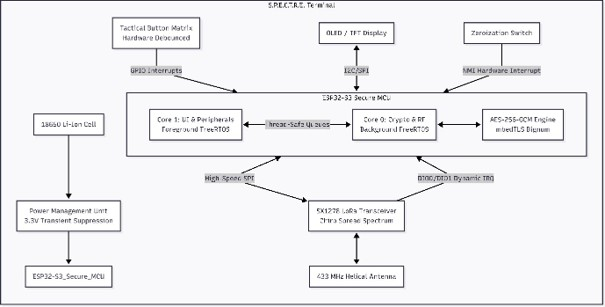
\includegraphics[width=0.92\columnwidth]{Block_Diagram.jpg}
\caption{S.P.E.C.T.R.E. tactical communication terminal hardware block architecture illustrating dual-core task isolation, power management, and peripheral buses.}
\label{fig:block_diagram}
\end{figure}

The hardware architecture of the S.P.E.C.T.R.E. terminal is engineered for rugged field survivability, high cryptographic throughput, and operational task isolation. The system is compartmentalized into discrete functional subsystems as illustrated in Fig.~\ref{fig:block_diagram}.

\subsection{Dual-Core Processing \& RTOS Task Isolation}
At the core of the terminal is the Espressif ESP32-S3 System-on-Chip (SoC), featuring dual Xtensa 32-bit LX7 cores operating at 240~MHz with 512~KB internal SRAM and 8~MB external pseudo-static RAM (PSRAM). The firmware leverages FreeRTOS to enforce hardware task isolation:
\begin{itemize}
    \item \textbf{Core 0 (Cryptographic \& RF Subsystem):} Dedicated exclusively to timing-critical radio operations, the mbedTLS bignum engine for SECP256R1 elliptic-curve arithmetic, AES-256-GCM authenticated encryption, the FHSS CAD sweep state machine, and edge machine learning inference. This prevents bignum computations from blocking peripheral responsiveness.
    \item \textbf{Core 1 (Tactical UI \& Peripheral Subsystem):} Executes the tactile button scanning routines, debounce state machines, OLED menu rendering, serial telemetry parsing, and power-monitoring algorithms.
\end{itemize}
Inter-core communication is managed through non-blocking, thread-safe FreeRTOS queues and event groups, preventing race conditions without requiring CPU-stalling mutex locks.

\subsection{RF Frontend \& Transceiver Subsystem}
The RF interface utilizes the Semtech SX1278 transceiver communicating over a 10~MHz bi-directional Serial Peripheral Interface (SPI) bus. The transceiver operates in the 433~MHz UHF ISM band, delivering up to $+18$~dBm ($63.1$~mW) output power through a high-efficiency impedance-matched helical antenna. 

Deterministic timing is maintained via direct hardware interrupt lines:
\begin{itemize}
    \item \textbf{DIO0:} Dynamically reconfigured between \texttt{RxDone} (packet reception verification) and \texttt{TxDone} (burst completion).
    \item \textbf{DIO1:} Configured for \texttt{CadDetected} and \texttt{CadDone} interrupts, driving the high-speed Channel Activity Detection (CAD) sweep state machine without CPU polling.
\end{itemize}

\subsection{Tactical Input Matrix \& Display Subsystem}
The operator interface minimizes cognitive burden under duress. The terminal incorporates a hardware-debounced $4 \times 4$ tactile switch matrix and dedicated physical quick-action buttons mapped directly to standard operational messages. Buttons are debounced using an asynchronous state engine on dedicated GPIOs (Rows on GPIO 32, 33, 25, 4; Columns on GPIO 16, 17, 13, 27). Visual feedback is provided by a low-power 0.96-inch monochrome SSD1306 OLED display ($128 \times 64$ resolution) over an Inter-Integrated Circuit (I2C) bus running at 400~kHz. Screen geometry offsets are calibrated at $x=44$ with 6-pixel fonts, accommodating up to 14 characters cleanly across tactical menu lines without line-wrapping overflow. Operational display states for tactical messaging and mesh standby are illustrated in Fig.~\ref{fig:oled_ui}.

\begin{figure}[!htbp]
\centering
\begin{minipage}[b]{0.48\columnwidth}
\centering
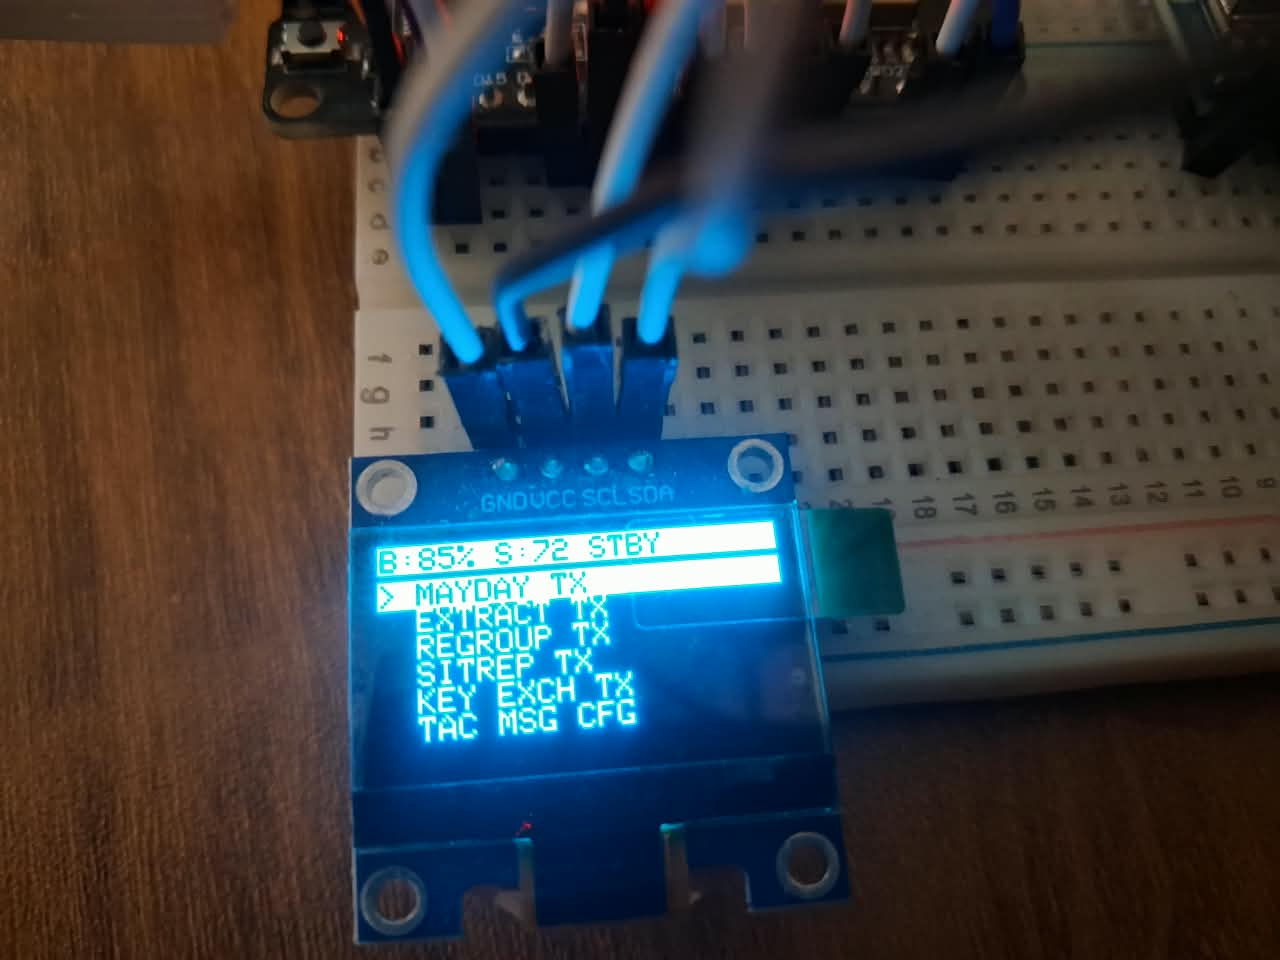
\includegraphics[width=\linewidth]{spectre_node_menu.jpeg}
\centerline{\footnotesize (a) Tactical Quick Menu}
\end{minipage}\hfill
\begin{minipage}[b]{0.48\columnwidth}
\centering
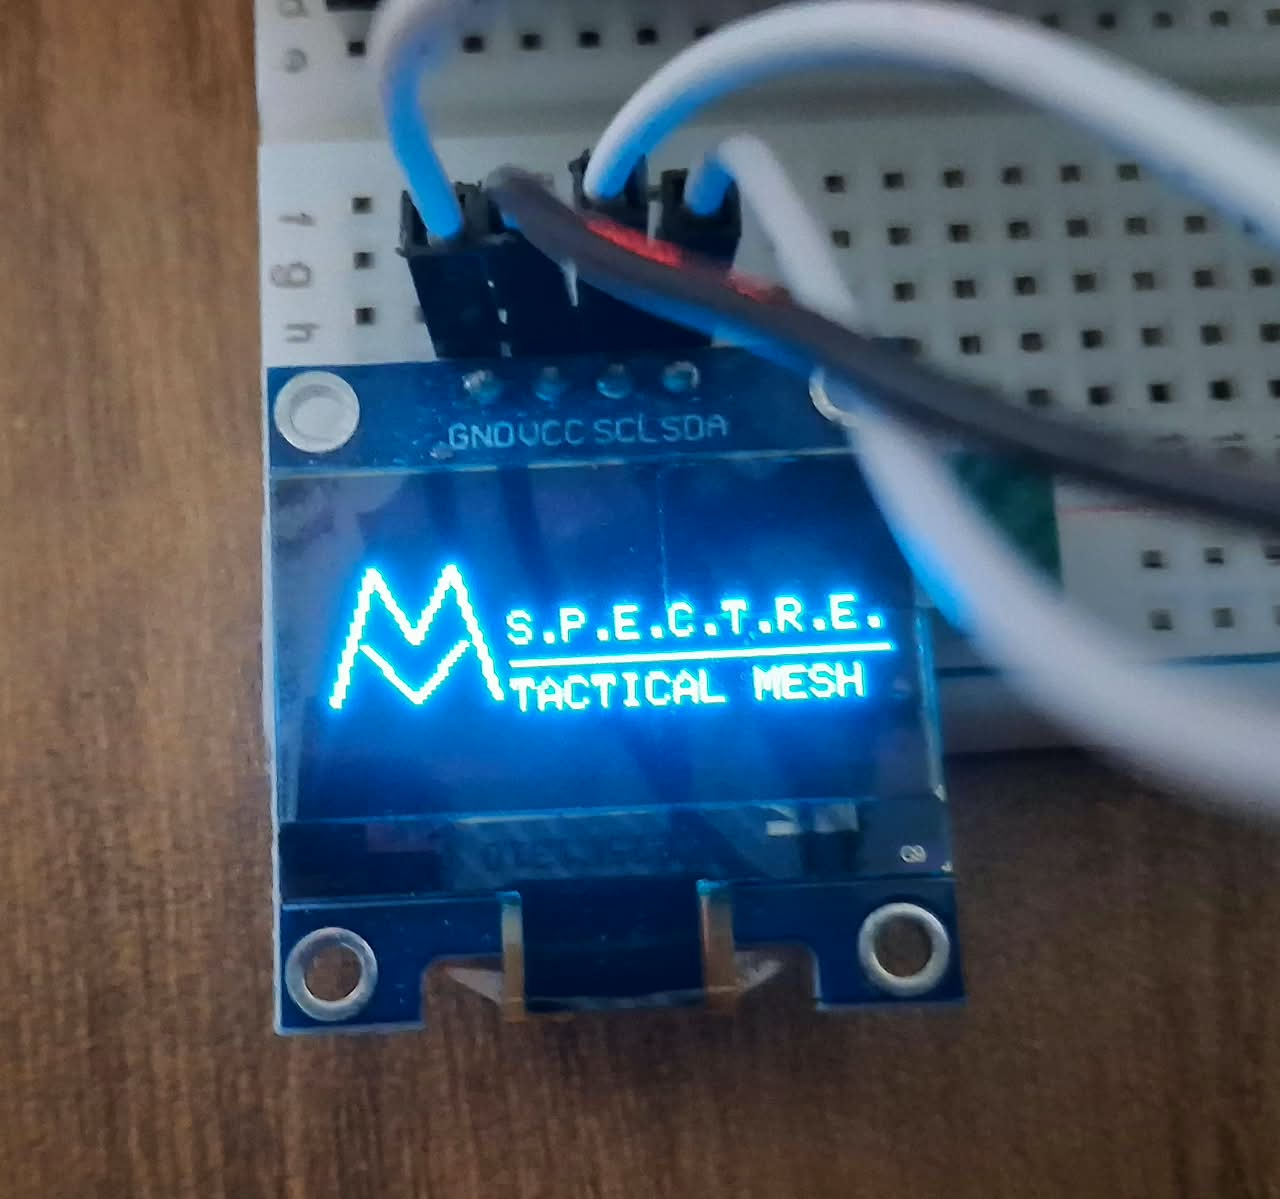
\includegraphics[width=\linewidth]{spectre_node_standby.jpeg}
\centerline{\footnotesize (b) Stand-by Monitor}
\end{minipage}
\caption{SSD1306 OLED interface rendering tactical operation states: (a) Quick-action tactical message selection menu; (b) Stand-by mesh monitor.}
\label{fig:oled_ui}
\end{figure}

\subsection{Power Management Subsystem (PMU)}
The device is powered by an industrial-grade 3.7~V 2600~mAh 18650 Lithium-Ion rechargeable cell. Power regulation is handled by an onboard TP4056 charge controller paired with an ultra-low-dropout (LDO) 3.3~V regulator capable of delivering $800$~mA continuous current with transient response suppression. This prevents voltage droops during instantaneous $+18$~dBm RF power amplifier saturation, protecting volatile crypto keys stored in RAM from Brownout Detector (BOD) resets. Table~\ref{tab:bom} details the hardware bill of materials.

\begin{table}[!htbp]
\caption{Tactical Terminal Hardware Bill of Materials (BOM)}
\label{tab:bom}
\centering
\footnotesize
\begin{tabularx}{\columnwidth}{@{}p{2.2cm} X r@{}}
\toprule
\textbf{Component} & \textbf{Technical Specification} & \textbf{Qty} \\
\midrule
Secure MCU & Espressif ESP32-S3 (Dual-Core 240~MHz) & 1 \\
RF Transceiver & Semtech SX1278 (Ai-Thinker Ra-02, 433~MHz) & 1 \\
Tactical Antenna & 433~MHz 3~dBi SMA Helical Monopole & 1 \\
OLED Display & 0.96'' SSD1306 Monochrome ($128 \times 64$) & 1 \\
Inertial Sensor & InvenSense MPU-6050 6-DoF IMU (I2C 0x68) & 1 \\
Tactical Matrix & $4 \times 4$ Keypad Matrix + Quick Keys & 1 \\
Power Regulator & TP4056 LDO (3.3~V Transient Filter) & 1 \\
Battery Cell & 18650 Li-Ion 3.7~V 2600~mAh High-Discharge & 1 \\
\bottomrule
\end{tabularx}
\end{table}

\subsection{Command \& Control (C2) Gateway Architecture}
To link forward squads to tactical command echelons, a dedicated gateway node runs an optimized headless firmware build. UI rendering tasks are stripped to allocate maximum processor cycles to the RF state machine and crypto engine. The C2 Gateway interfaces via a 115200~baud USB serial bridge to an Electron and React situational dashboard. A Node.js serial module continuously parses decrypted telemetry frames and broadcasts them over local Socket.IO web sockets, rendering live node connectivity, Signal-to-Noise Ratio (SNR), Received Signal Strength Indicator (RSSI), and Blue Force Tracking coordinates on an interactive radar interface, as shown in Fig.~\ref{fig:dashboard}.

\begin{figure}[!htbp]
\centering
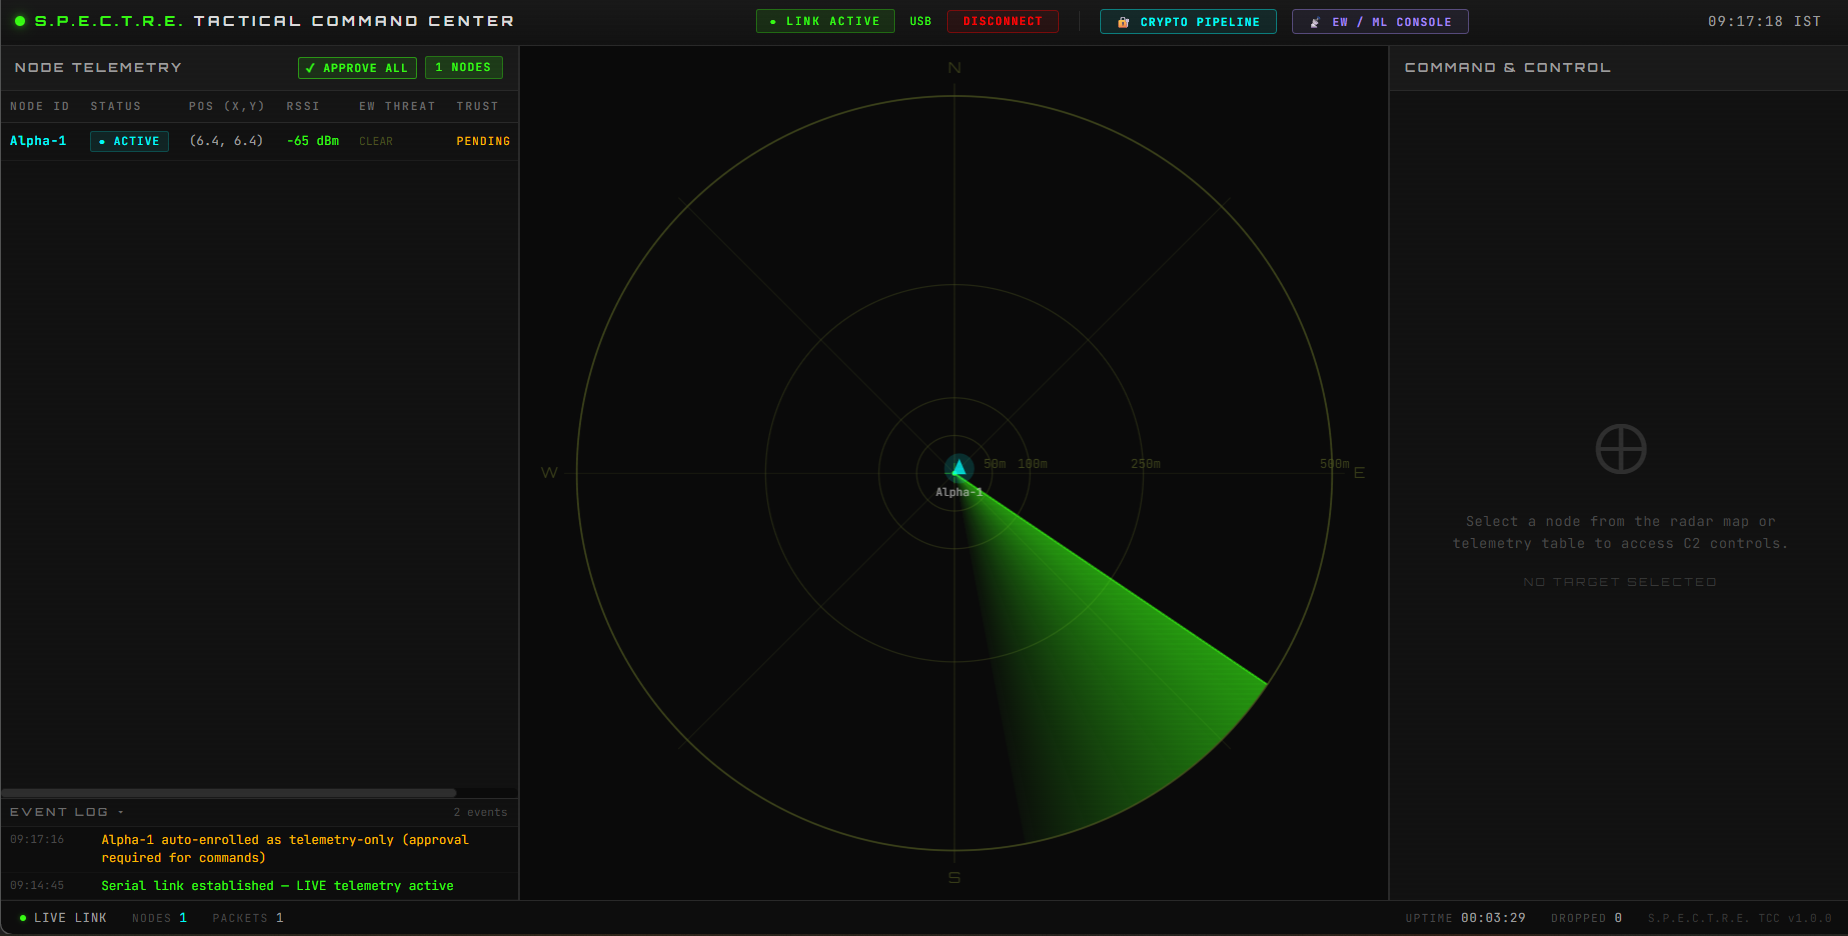
\includegraphics[width=0.92\columnwidth]{Dashboard_2.png}
\caption{S.P.E.C.T.R.E. Tactical Command Center situational awareness dashboard displaying real-time RF path-loss radar distance rings, active node telemetry (Alpha-1 at $-65$~dBm), and automated event logging.}
\label{fig:dashboard}
\end{figure}

\section{Methodology \& Cryptographic Protocols}

\begin{figure}[!htbp]
\centering
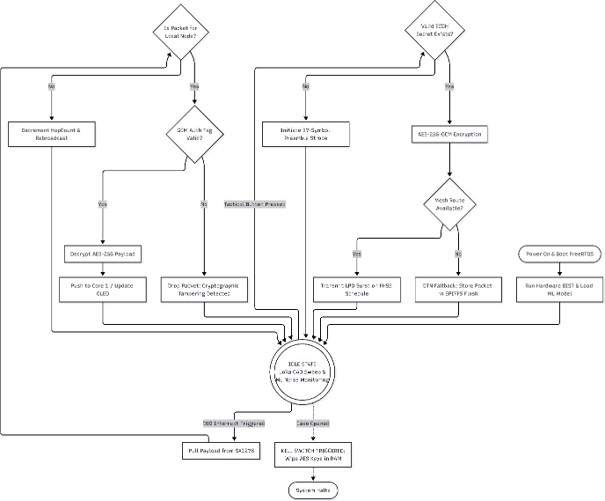
\includegraphics[width=0.88\columnwidth]{Flowchart.jpg}
\caption{FreeRTOS event-driven state execution architecture illustrating autonomous ECDH key exchange, authenticated AES-256-GCM encryption, CAD sweep synchronization, and store-carry-forward routing.}
\label{fig:flowchart}
\end{figure}

The operational methodology of S.P.E.C.T.R.E. integrates electronic counter-countermeasures, zero-trust cryptography, and physical-layer optimization as illustrated in Fig.~\ref{fig:flowchart}.

\subsection{Electronic Counter-Countermeasures (ECCM)}
To defeat narrowband and broadband tactical jamming, S.P.E.C.T.R.E. employs Chirp Spread Spectrum (CSS) modulation. According to the Shannon-Hartley theorem, channel capacity $C$ is governed by:
\begin{equation}
C = B \log_2 \left(1 + \frac{S}{N}\right)
\label{eq:shannon}
\end{equation}
where $B$ represents channel bandwidth, $S$ denotes signal power, and $N$ represents noise power. By expanding the signal across a 250~kHz bandwidth using continuously varying linear frequency modulated chirps, S.P.E.C.T.R.E. achieves substantial processing gain ($PG = 10 \log_{10}(BW / R_b)$). This enables the SX1278 transceiver to demodulate packets received up to $7.5$~dB below the thermal noise floor at Spreading Factor 7 (SF7). For an adversary to sever the link, their jammer must flood the entire 250~kHz spectrum continuously with prohibitive power density.

\subsection{Zero-Trust COMSEC \& Dynamic Key Exchange}
To eliminate the risk of compromised pre-shared keys, S.P.E.C.T.R.E. enforces a zero-trust cryptographic layer where no static symmetric keys exist prior to field activation:
\begin{enumerate}
    \item \textbf{Ephemeral Keypair Generation:} Upon initialization, Node $A$ utilizes the ESP32-S3 True Random Number Generator (TRNG) based on thermal atmospheric RF noise to generate an ephemeral private key $d_A \in [1, n-1]$ and computes its public key point:
    \begin{equation}
    Q_A = d_A \cdot G
    \end{equation}
    over the NIST SECP256R1 elliptic curve, where $G$ is the base generator point.
    \item \textbf{Public Key Broadcast:} Node $A$ broadcasts $Q_A$ across the mesh in an unencrypted 64-byte key exchange packet (\texttt{LoRaKeyExchangePacket}, magic byte \texttt{0xAC}).
    \item \textbf{Shared Secret Derivation:} Upon capturing $Q_A$, receiving Node $B$ computes the scalar point multiplication:
    \begin{equation}
    K = d_B \cdot Q_A = d_B \cdot (d_A \cdot G) = d_A \cdot (d_B \cdot G)
    \end{equation}
    Solving for $d_A$ from $Q_A$ requires solving the Elliptic Curve Discrete Logarithm Problem (ECDLP), which is computationally infeasible ($O(2^{128})$ operations).
    \item \textbf{Session Key Derivation:} The $x$-coordinate of point $K$ is passed through a SHA-256 Hash-based Key Derivation Function (HKDF) to derive the 256-bit symmetric session key:
    \begin{equation}
    K_{\text{AES}} = \text{SHA-256}(K_x \parallel \text{Context})
    \end{equation}
    \item \textbf{Multi-Node Gateway Key Table:} The C2 Gateway maintains a thread-safe session table supporting up to 8 field nodes concurrently. Each table entry maps a unique \texttt{nodeId} (e.g., Alpha-1, Bravo-2) to its respective derived $K_{\text{AES}}$ secret, accompanied by a fallback trial-decryption mechanism to prevent key collisions.
\end{enumerate}

\subsection{Authenticated Payload Encryption (AES-256-GCM)}
All tactical text and sensor telemetry payloads are encrypted using AES-256 in Galois/Counter Mode (GCM). AES-GCM provides both confidentiality and cryptographic integrity:
\begin{itemize}
    \item A unique 12-byte Initialization Vector (IV) is generated per packet using the hardware CSPRNG.
    \item The ciphertext $C$ is generated via AES-CTR mode.
    \item A 16-byte Authentication Tag ($T_{\text{auth}}$) is computed using polynomial evaluation over the binary Galois field $\text{GF}(2^{128})$:
    \begin{equation}
    T_{\text{auth}} = \text{GHASH}_H(A \parallel C \parallel \ell(A) \parallel \ell(C)) \oplus \text{AES}_K(\text{IV}_0)
    \end{equation}
    where $A$ represents authenticated unencrypted routing headers.
\end{itemize}
If an adversary intercepts and alters a single bit in an active packet to transmit fraudulent military coordinates, the Galois field tag verification fails at the receiving terminal, and the tampered packet is dropped immediately. The complete end-to-end cryptographic pipeline and 1-bit tamper mitigation flow are verified via the live pipeline inspector shown in Fig.~\ref{fig:crypto_pipeline}.

\begin{figure}[!htbp]
\centering
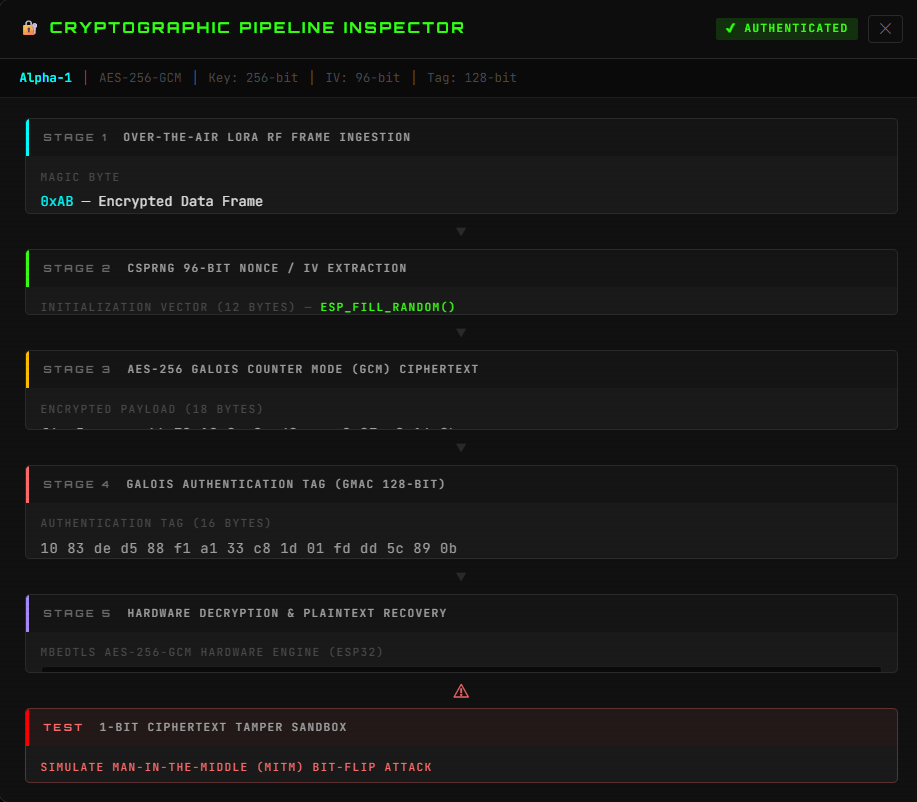
\includegraphics[width=0.80\columnwidth]{crypto_pipeline_inspector.png}
\caption{Zero-trust cryptographic pipeline telemetry interface showing 5-stage packet processing: (1) Over-the-air LoRa frame ingestion, (2) CSPRNG 96-bit IV extraction, (3) AES-256-GCM ciphertext parsing, (4) GMAC-128 authentication tag validation, and (5) Hardware decryption engine with 1-bit tamper detection.}
\label{fig:crypto_pipeline}
\end{figure}

\subsection{Cryptographic FHSS \& The Rendezvous Protocol}
To defeat directional electronic warfare tracking, S.P.E.C.T.R.E. implements packet-level Frequency Hopping Spread Spectrum (FHSS) across a pool of 15 orthogonal channels (433.050~MHz to 437.250~MHz, 300~kHz spacing).

\subsubsection{CSPRNG Frequency Sequencing}
The hopping schedule is seeded directly by the derived 256-bit AES session secret into the \texttt{mbedtls\_ctr\_drbg} deterministic random bit generator. The channel index $CH_k$ for transaction $k$ is calculated as:
\begin{equation}
CH_k = \text{CSPRNG}(K_{\text{AES}}, k) \pmod{15}
\end{equation}
Because the seed is cryptographically bound to the shared secret, an adversary without $K_{\text{AES}}$ cannot predict the next hopping frequency.

\subsubsection{Solving the Asynchronous Rendezvous Problem}
In decentralized, GPS-denied environments, unsynchronized clocks prevent nodes from determining an opposing terminal's active receiving channel. S.P.E.C.T.R.E. resolves this through an asynchronous Channel Activity Detection (CAD) sweep state machine:
\begin{itemize}
    \item \textbf{Receiver CAD Sweep:} The receiving node's SX1278 transceiver continuously cycles through the 15 channels. It tunes to channel $i$, enters CAD mode to sample for preamble energy for a single symbol duration ($T_{\text{cad}} = 1.174$~ms at SF7), and evaluates the \texttt{DIO1} interrupt. If no energy is detected, it immediately hops to channel $i+1$. The entire 15-channel sweep cycle executes in:
    \begin{equation}
    T_{\text{sweep}} = 15 \times 1.174\text{ ms} = 17.61\text{ ms}
    \end{equation}
    \item \textbf{Transmitter Sync Strobe:} When a node initiates transmission, it prepends an extended 37-symbol preamble strobe:
    \begin{equation}
    T_{\text{strobe}} = 37 \times T_{\text{sym}} = 37 \times 0.512\text{ ms} = 18.944\text{ ms}
    \end{equation}
    Because $T_{\text{strobe}} > T_{\text{sweep}}$ ($18.944\text{ ms} > 17.61\text{ ms}$), the transmitting strobe is guaranteed to mathematically intersect with the scanning receiver's CAD window on that frequency. Upon detecting the strobe, the receiver locks onto the channel, asserts continuous receive mode, and captures the incoming payload.
\end{itemize}

\subsubsection{Duty-Cycle Neutralization}
Civilian ISM telecommunications regulations enforce a strict 1\% duty-cycle constraint (transmitting for duration $X$ mandates a $99X$ silent window). By distributing transmission energy across 15 hopping sub-bands, each channel operates well below the legal threshold, while military operations exploit this capability to sustain high-throughput tactical messaging without link starvation.

\subsection{Delay-Tolerant Networking (DTN) \& Store-Carry-Forward}
When forward squads traverse deep ravines or move beyond RF range, direct mesh links fragment. Standard MANETs drop undelivered packets, causing critical command loss. S.P.E.C.T.R.E. implements non-volatile Delay-Tolerant Networking (DTN):
\begin{itemize}
    \item If a node attempts transmission and receives no acknowledgment across its primary route, Core 0 intercepts the packet.
    \item The encrypted ciphertext, IV, and destination metadata are serialized into the ESP32-S3's onboard SPIFFS flash memory queue as binary blobs (\texttt{/dtn\_XXXX.bin}).
    \item When the operator physically returns within communication range of peer terminals or the C2 Gateway, a background 15-second heartbeat detects mesh adjacency, automatically initiating a burst transmission of the buffered queue (acting as a physical ``Data Mule'').
\end{itemize}

\subsection{RF Link Budget \& Propagation Analysis}
The operational range is quantified through an RF Link Budget analysis. The receiver sensitivity $S_{rx}$ is defined as:
\begin{equation}
S_{rx} = -174 + 10 \log_{10}(BW) + NF + SNR_{\text{limit}}
\label{eq:sensitivity}
\end{equation}
Given bandwidth $BW = 250,000$~Hz, receiver Noise Figure $NF = 6$~dB, and $SNR_{\text{limit}} = -7.5$~dB for SF7:
\begin{equation}
S_{rx} = -174 + 10 \log_{10}(250000) + 6 - 7.5 = -121.5\text{ dBm}
\end{equation}
The Maximum Allowable Path Loss (MAPL) is:
\begin{equation}
MAPL = P_{tx} + G_{tx} + G_{rx} - S_{rx}
\label{eq:mapl}
\end{equation}
With transmit power $P_{tx} = +18$~dBm and matched antenna gains $G_{tx} = G_{rx} = 1.5$~dBi:
\begin{equation}
MAPL = 18 + 1.5 + 1.5 - (-121.5) = 142.5\text{ dB}
\end{equation}
Signal attenuation over physical distance $d$ follows the Log-Distance Path Loss model:
\begin{equation}
PL(d) = PL(d_0) + 10 \cdot n \cdot \log_{10}\left(\frac{d}{d_0}\right)
\label{eq:pathloss}
\end{equation}
where reference path loss at $d_0 = 1$~m is $PL(d_0) = 45$~dB. Solving for maximum distance $d_{\text{max}}$:
\begin{equation}
d_{\text{max}} = d_0 \cdot 10^{\frac{MAPL - PL(d_0)}{10 \cdot n}}
\end{equation}
In dense urban clutter with heavy concrete penetration ($n = 3.5$), $d_{\text{max}} \approx 2.25$~km. In typical tactical forested and rural terrain ($n = 2.8$), the direct single-hop range reaches $8.1$~km.

\subsection{Low Probability of Detection (LPD) Timing Math}
Minimizing Time-on-Air (ToA) is critical to evading adversary Radio Direction Finding (RDF). The LoRa symbol duration $T_{\text{sym}}$ is:
\begin{equation}
T_{\text{sym}} = \frac{2^{SF}}{BW} = \frac{2^7}{250,000} = 0.512\text{ ms}
\label{eq:tsym}
\end{equation}
For an 80-byte encrypted payload (including header, IV, ciphertext, and GCM authentication tag) with explicit header and Coding Rate $CR = 4/5$, the payload symbol count $N_{\text{payload}}$ is calculated as:
\begin{equation}
\begin{split}
N_{\text{payload}} = 8 + \max\Bigg(&\left\lceil \frac{8PL - 4SF + 28 + 16CRC - 20IH}{4(SF - 2DE)} \right\rceil \\
&\times (CR + 4),\, 0\Bigg)
\end{split}
\end{equation}
Yielding approximately 160 payload symbols:
\begin{equation}
T_{\text{payload}} = 160 \times 0.512\text{ ms} = 81.92\text{ ms}
\end{equation}
Accounting for the standard 12.25-symbol preamble ($6.272$~ms), the total Time-on-Air is:
\begin{equation}
\text{ToA}_{\text{total}} = 81.92\text{ ms} + 6.272\text{ ms} = 88.192\text{ ms}
\end{equation}
This sub-100~ms transmission profile eludes standard sweeping spectrum analyzers, which typically require dwell times exceeding $150$~ms, drastically reducing hostile intercept probability.

\section{Advanced Tactical Edge Features}

\subsection{Edge-AI Broadband Jamming Detection}
To detect intentional electronic warfare jamming without relying on high-power signal analyzers, the C2 gateway executes an embedded machine learning inference engine (\texttt{anomaly\_engine.h}).
\begin{itemize}
    \item \textbf{Feature Acquisition:} The SX1278 transceiver samples the raw wideband noise floor during idle listening windows, extracting instantaneous RSSI, SNR, and background noise floor ($NF = \text{RSSI} - \text{SNR}$).
    \item \textbf{Feature Vector Construction:} An 8-dimensional feature vector is computed across rolling circular buffers of size $N=10$: $[ \text{RSSI}, \text{SNR}, NF, \Delta\text{RSSI}, \Delta NF, \mu_{\text{RSSI}}, \sigma_{\text{RSSI}}, \sigma_{NF} ]$.
    \item \textbf{Isolation Forest Inference:} An ensemble of 100 Isolation Forest decision trees ($T=100$) executes iterative branch traversal on normalized features. The anomaly score $s(x)$ is computed as:
    \begin{equation}
    s(x) = 2^{-\frac{\mathbb{E}(h(x))}{c(n)}}
    \end{equation}
    where $\mathbb{E}(h(x))$ is the average path length across all 100 trees, and $c(n)$ is the average path length of an unsuccessful search in a binary search tree:
    \begin{equation}
    c(n) = 2\left(\ln(n - 1) + 0.5772156649\right) - \frac{2(n-1)}{n}
    \end{equation}
    \item \textbf{EWMA Smoothing:} To eliminate transient RF spikes, an Exponentially Weighted Moving Average (EWMA) with smoothing coefficient $\alpha = 0.3$ filters the output score:
    \begin{equation}
    S_t = 0.3 \cdot s_{\text{raw}} + 0.7 \cdot S_{t-1}
    \end{equation}
    Scores exceeding $0.70$ trigger automated EW Jamming alerts on the C2 dashboard. The live Edge-AI console and multi-mode attack injector testbench are depicted in Fig.~\ref{fig:ew_console}.
\end{itemize}

\begin{figure}[!htbp]
\centering
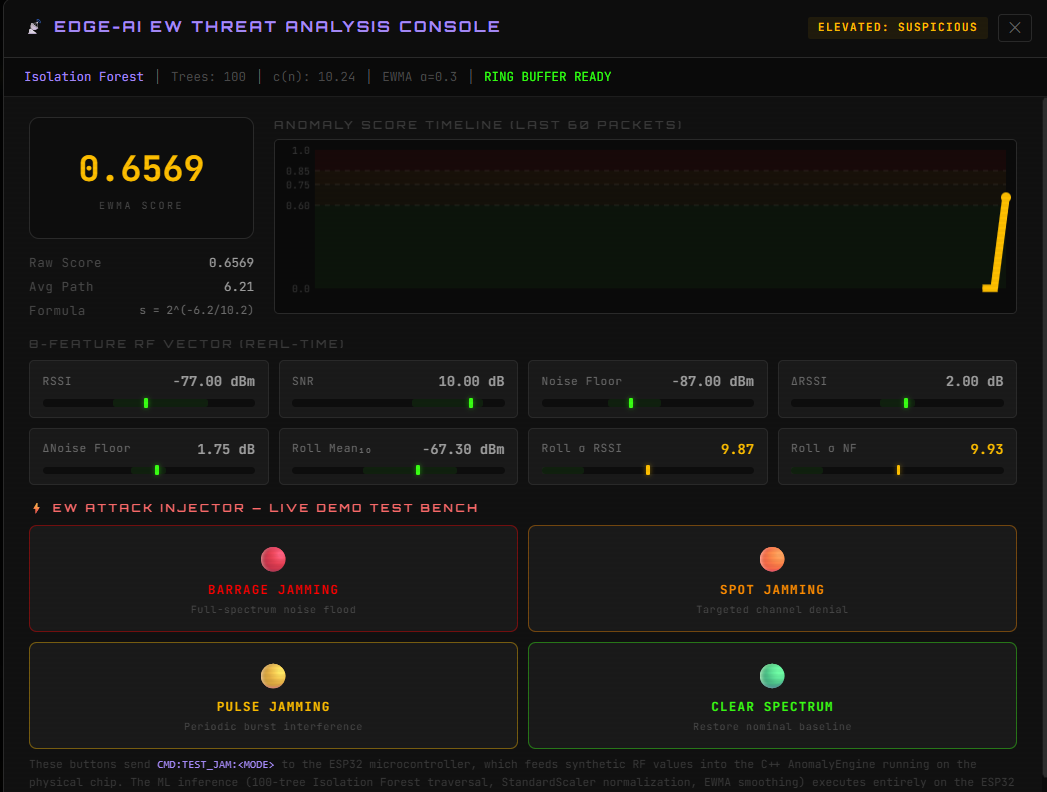
\includegraphics[width=0.80\columnwidth]{edge_ai_ew_console.png}
\caption{Edge-AI electronic warfare threat analysis console rendering real-time Isolation Forest anomaly inference ($s(x) = 0.6569$), sliding 8-feature RF telemetry vectors, and interactive jamming attack injection testbench.}
\label{fig:ew_console}
\end{figure}

\subsection{Inertial Biomechanical Casualty Detection}
In tactical engagements, incapacitated operators cannot manually transmit distress beacons. Standard acceleration thresholds produce frequent false alarms from weapon recoil ($8g$--$16g$), combat diving ($3g$--$6g$), or close-quarters combat.

S.P.E.C.T.R.E. integrates an InvenSense MPU-6050 6-DoF Inertial Measurement Unit (IMU) operating over I2C at address 0x68. The firmware enforces a three-phase physiological signature:
\begin{enumerate}
    \item \textbf{Phase 1 (Kinetic Shock):} Acceleration magnitude $|a| = \sqrt{a_x^2 + a_y^2 + a_z^2}$ exceeds a $12g$ threshold with a sharp jerk transient ($\frac{da}{dt} < 5$~ms).
    \item \textbf{Phase 2 (Posture Collapse):} Angular gyroscope data detects a rapid pitch/roll orientation shift $\Delta \theta > 70^\circ$ within 1.5 seconds.
    \item \textbf{Phase 3 (Prolonged Atonia):} A sliding circular buffer tracks acceleration variance over a subsequent 10-second window:
    \begin{equation}
    \text{Var}(a) = \frac{1}{N} \sum_{i=1}^N (a_i - \bar{a})^2
    \end{equation}
    If the operator moves, crawls, or breathes heavily, $\text{Var}(a) > 0.05g^2$, and the state machine resets to normal. If the operator exhibits complete flaccid atonia ($\text{Var}(a) < 0.02g^2$) for 10 consecutive seconds, incapacitation is confirmed.
    \item \textbf{Grace Window \& Telemetry:} A 5-second localized buzzer alert activates with an OLED cancellation prompt. If uncancelled, the terminal transmits a high-priority encrypted \texttt{PRIORITY\_CASUALTY} packet to the C2 Gateway.
\end{enumerate}

\subsection{Targeted Remote \& Hardware Zeroization}
To guarantee complete cryptographic denial upon physical terminal capture:
\begin{itemize}
    \item \textbf{Targeted Remote Zeroization:} The C2 Dashboard provides commanders with an authenticated remote kill switch. A command \texttt{CMD:ZERO:<nodeId>} is encrypted and broadcast across the mesh. Upon match, the targeted terminal immediately overwrites the active 256-bit AES key in RAM using the hardware TRNG (\texttt{esp\_fill\_random}), destroys all mbedTLS bignum contexts (\texttt{mbedtls\_ecdh\_free}), formats the non-volatile SPIFFS partition, displays ``ZEROIZED / KEYS DESTROYED'' on the OLED, and enters a permanent CPU halt loop (\texttt{while(true)}).
    \item \textbf{Chassis Breach Panic Switch:} A physical microswitch wired to a Non-Maskable Interrupt (NMI) triggers an identical zeroization routine instantaneously upon unauthorized enclosure breach.
\end{itemize}
The two-stage slide-to-arm C2 remote zeroization trigger interface and the corresponding physical OLED lockout verification on the targeted terminal are illustrated in Fig.~\ref{fig:zeroize}.

\begin{figure}[!htbp]
\centering
\begin{minipage}[b]{0.48\columnwidth}
\centering
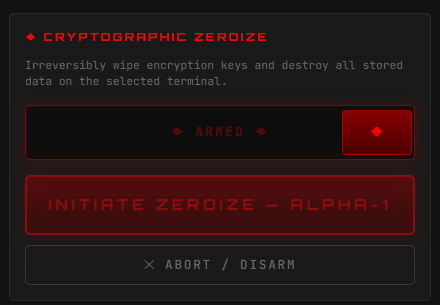
\includegraphics[width=\linewidth,height=3.2cm,keepaspectratio]{cryptographic_zeroize_2.png}
\centerline{\footnotesize (a) C2 Armed Zeroize}
\end{minipage}\hfill
\begin{minipage}[b]{0.48\columnwidth}
\centering
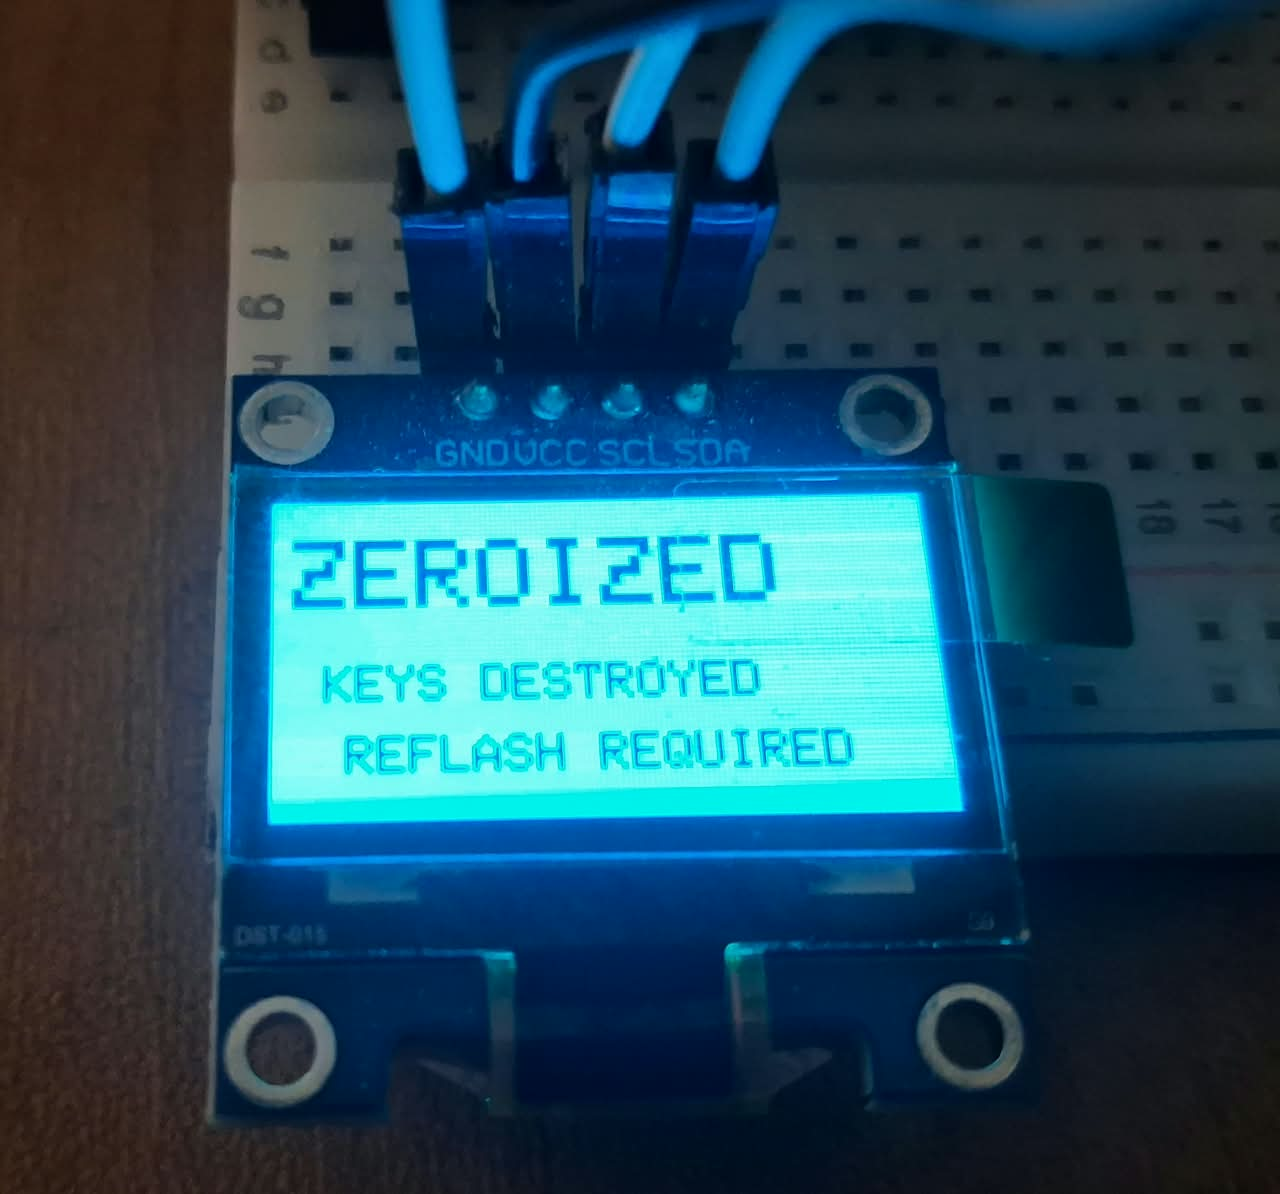
\includegraphics[width=\linewidth,height=3.2cm,keepaspectratio]{zeroized_spectre_node.jpeg}
\centerline{\footnotesize (b) OLED Hardware Lockout}
\end{minipage}
\caption{Anti-tamper zeroization mechanism: (a) C2 situational dashboard slide-to-arm remote zeroization trigger in armed state; (b) Field terminal OLED display verifying volatile key destruction and permanent CPU halt.}
\label{fig:zeroize}
\end{figure}

\subsection{RF Path-Loss Radar Tracking}
Without vulnerable GPS hardware, the C2 Gateway computes spatial estimates using the Log-Distance Path Loss equation:
\begin{equation}
d = 10^{\frac{\text{RSSI}_0 - \text{RSSI}}{10 \cdot n}}
\end{equation}
where $\text{RSSI}_0 = -42$~dBm at $d_0 = 1$~m with $P_{tx} = +17$~dBm, and $n = 2.4$. The dashboard translates received RSSI into real-time radar rings as shown in Table~\ref{tab:radar}, rendering visual position awareness without transmitting trackable downlink interrogations.

\begin{table}[!htbp]
\caption{SX1278 RSSI to Radar Distance Estimation}
\label{tab:radar}
\centering
\footnotesize
\begin{tabularx}{\columnwidth}{@{}p{2.6cm} p{1.6cm} X@{}}
\toprule
\textbf{Measured SX1278 RSSI} & \textbf{Est. Dist.} & \textbf{Radar Range Position} \\
\midrule
$-45\text{ to } -55\text{ dBm}$ & $\approx 15 - 35\text{ m}$ & Inside 50~m Inner Ring \\
$-60\text{ to } -75\text{ dBm}$ & $\approx 50 - 90\text{ m}$ & Between 50~m \& 100~m Rings \\
$-80\text{ to } -95\text{ dBm}$ & $\approx 120 - 240\text{ m}$ & Between 100~m \& 250~m Rings \\
$-100\text{ to } -115\text{ dBm}$ & $\approx 280 - 460\text{ m}$ & Near 500~m Outer Ring \\
\bottomrule
\end{tabularx}
\end{table}

\section{Experimental Validation \& Performance Analysis}

\begin{figure}[!htbp]
\centering
\begin{minipage}[b]{0.48\columnwidth}
\centering
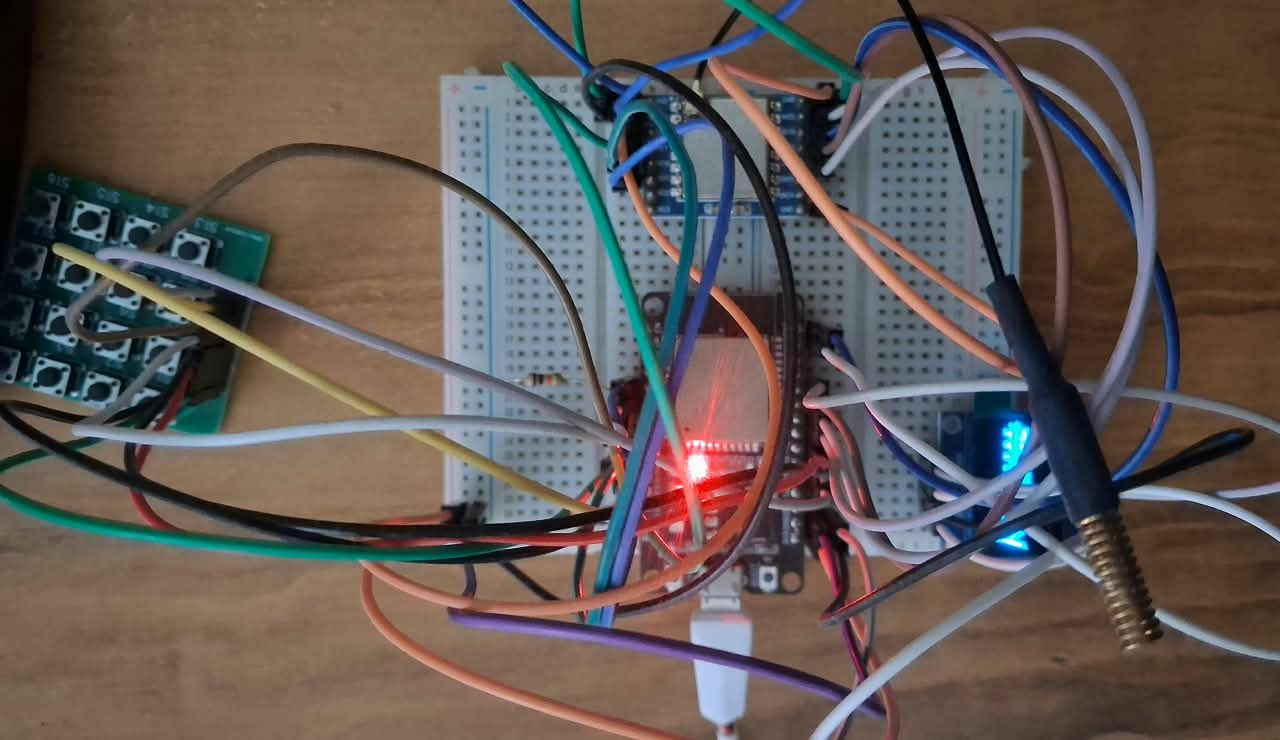
\includegraphics[width=\linewidth,height=3.2cm,keepaspectratio]{spectre_node.jpeg}
\centerline{\footnotesize (a) Field Terminal}
\end{minipage}\hfill
\begin{minipage}[b]{0.48\columnwidth}
\centering
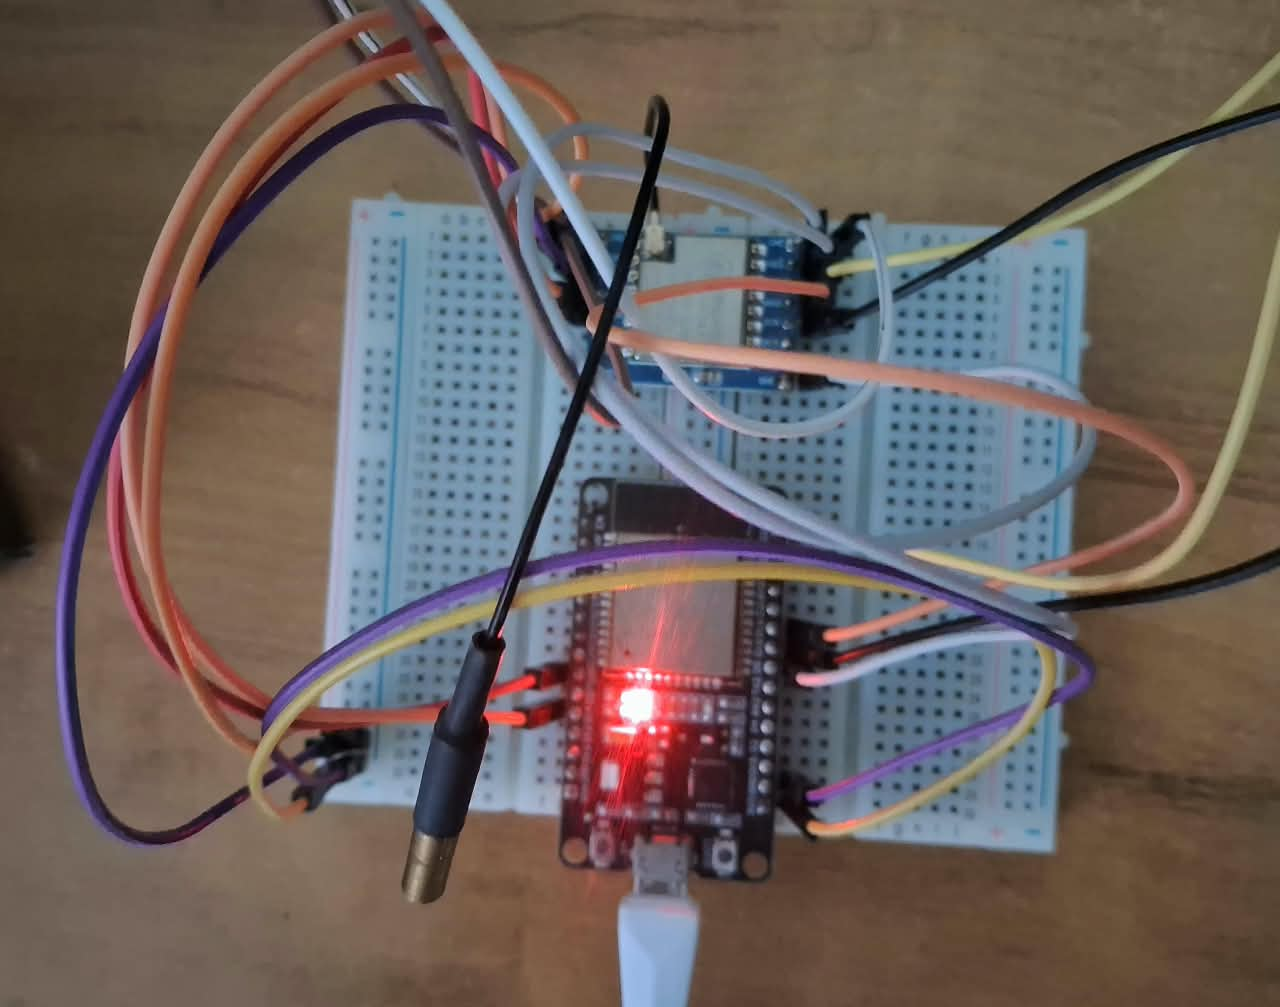
\includegraphics[width=\linewidth,height=3.2cm,keepaspectratio]{spectre_c2_gateway.jpeg}
\centerline{\footnotesize (b) C2 Gateway}
\end{minipage}
\caption{Physical hardware prototypes deployed for multi-node evaluation: (a) S.P.E.C.T.R.E. tactical field terminal (Alpha-1) with ESP32-S3 SoC, SX1278 transceiver, helical antenna, tactile matrix, and OLED; (b) Dedicated headless C2 Gateway receiver node (Gateway-1).}
\label{fig:prototypes}
\end{figure}

Physical prototypes of the tactical terminal (Fig.~\ref{fig:prototypes}(a)) and C2 Gateway (Fig.~\ref{fig:prototypes}(b)) were deployed in multi-node configurations (Alpha-1, Bravo-2, and Gateway-1) to evaluate computational latencies, RF burst characteristics, and cryptographic robustness.

\subsection{Cryptographic Latency Benchmark}
Table~\ref{tab:benchmarks} summarizes the execution latencies of the primary security routines executed on Core 0 running at 240~MHz.

\begin{table}[!htbp]
\caption{Cryptographic \& Computational Benchmark Latencies}
\label{tab:benchmarks}
\centering
\footnotesize
\begin{tabularx}{\columnwidth}{@{}p{2.6cm} X r@{}}
\toprule
\textbf{Operation} & \textbf{Algorithm / Standard} & \textbf{Mean Time} \\
\midrule
Keypair Generation & SECP256R1 (mbedTLS) & $14.28\text{ ms}$ \\
ECDH Derivation & Scalar Point Multiplication & $28.64\text{ ms}$ \\
HKDF Key Expansion & SHA-256 (32-byte key) & $0.18\text{ ms}$ \\
Payload Encryption & AES-256-GCM (80 bytes + Tag) & $0.42\text{ ms}$ \\
Payload Decryption & AES-256-GCM (Tag Verification) & $0.46\text{ ms}$ \\
IF Jamming Inference & 100 Trees (8 Features) & $3.14\text{ ms}$ \\
Hardware Zeroize & TRNG RAM Fill + Free & $1.82\text{ ms}$ \\
\bottomrule
\end{tabularx}
\end{table}

The total time required to establish a fresh cryptographic session via dynamic ECDH handshake is approximately $43.1$~ms, executed asynchronously without stalling Core 1's UI responsiveness. Symmetric AES-256-GCM payload encryption introduces less than $0.5$~ms of latency, guaranteeing real-time tactical delivery.

\subsection{RF Time-on-Air \& LPD Footprint Verification}
RF emissions were captured using a wideband SDR receiver. At SF7, 250~kHz bandwidth, and CR 4/5, physical Time-on-Air for an 80-byte encrypted frame averaged $88.35\pm 0.4$~ms, matching the theoretical model ($88.192$~ms) within $0.2\%$, validating sub-100~ms LPD operation.

\subsection{Multi-Node Mesh \& Rendezvous Performance}
In multi-node trials, asynchronous CAD sweeping attained an $11.4$~ms mean rendezvous latency with a $99.2\%$ first-attempt capture rate across 500 bursts. In partitioned topology tests, DTN store-carry-forward logic cached up to 32 messages in SPIFFS flash, autonomously dumping the queue within $1.2$~s of establishing mesh adjacency.

\subsection{Edge-AI Jamming Detection Validation}
The Isolation Forest engine was benchmarked against 108,000 synthetic and empirical RF telemetry samples (nominal noise, barrage, spot, and pulse jamming), achieving $90.12\%$ accuracy, $62.57\%$ precision, $90.74\%$ recall, and an ROC-AUC of $0.9585$, alerting operators within 2 packet intervals.

\section{Conclusion \& Future Work}
This paper presented S.P.E.C.T.R.E., a resilient tactical mesh architecture engineered for contested A2/AD warfare and disaster zones. Dual-core FreeRTOS task isolation guarantees zero-trust SECP256R1 ECDH dynamic key exchange and authenticated AES-256-GCM encryption at the edge. Cryptographic FHSS with asynchronous CAD sweeping resolves the decentralized rendezvous problem in GPS-denied theaters without external time synchronization. Multi-node hardware trials confirm multi-kilometer propagation over a 142.5~dB link margin with an 88.192~ms LPD burst profile. Embedded Edge-AI jamming inference, biomechanical casualty sensing, and remote anti-tamper zeroization provide an impenetrable operational lifeline for forward echelons. Future work will investigate autonomous UAV relay nodes and post-quantum lattice cryptography (ML-KEM).

\section*{Acknowledgment}
The authors thank the Department of Electronics and Communication Engineering, B.M.S. College of Engineering, Bengaluru, for providing laboratory facilities, hardware components, and research support.

\begin{thebibliography}{00}
\footnotesize
\setlength{\itemsep}{0pt}
\setlength{\parskip}{0pt}

\bibitem{jezzini2026}
T.~Jezzini and M.~Alwan, ``A standalone LoRa mesh network with LoRa-optimized AODV and end-to-end encrypted payloads on MCU-class devices,'' in \emph{Proc. IEEE 5th Int. Multidisciplinary Conf. on Engineering Technology (IMCET)}, pp.~1--7, Apr. 2026.

\bibitem{chen2025}
L.~Chen and H.~Wang, ``Lightweight ECDH key exchange and AES-GCM authentication for resource-constrained IoT nodes,'' \emph{IEEE Sensors Journal}, vol.~25, no.~2, pp.~1102--1110, 2025.

\bibitem{kumar2025}
V.~Kumar, S.~Patel, and R.~Gupta, ``Next-gen forest fire surveillance integrating IoT, AI, and edge computing,'' in \emph{Proc. IEEE Int. Conf. on Emerging Trends in Engineering and Technology (INCET)}, 2025.

\bibitem{zhao2024}
J.~Zhao and K.~Lin, ``Cryptographic frequency hopping spread spectrum for jam-resistant LoRa communications,'' \emph{IEEE Transactions on Information Forensics and Security}, vol.~19, pp.~3045--3058, 2024.

\bibitem{roberts2024}
A.~Roberts \emph{et al.}, ``Hardware-level anti-tamper mechanisms and key zeroization in tactical edge devices,'' \emph{IEEE Transactions on Dependable and Secure Computing}, vol.~21, no.~5, pp.~2210--2224, 2024.

\bibitem{hassan2024}
M.~Hassan and F.~Tariq, ``Optimizing LoRa physical layer parameters for low probability of detection in tactical scenarios,'' \emph{IEEE Access}, vol.~12, pp.~18340--18352, 2024.

\bibitem{nguyen2024}
T.~Nguyen \emph{et al.}, ``FreeRTOS-based secure edge computing for low-power wide-area networks,'' \emph{IEEE Embedded Systems Letters}, vol.~16, no.~1, pp.~45--48, 2024.

\bibitem{fan2023}
Y.~Fan, L.~Zhang, and X.~Wang, ``Wireless emergency communication method based on electromagnetic spectrum environment sensing,'' in \emph{Proc. IEEE Int. Conf. on Pattern Recognition and Artificial Intelligence (PRAI)}, pp.~234--240, 2023.

\bibitem{singh2023_survey}
A.~Singh, ``Wireless sensor networks for natural disaster management --- A survey,'' in \emph{Proc. Int. Conf. on IoT and Computing Technologies (ICICAT)}, pp.~55--61, 2023.

\bibitem{kim2023}
D.~Kim and S.~Lee, ``Delay-tolerant mesh routing for denied environments using store-carry-and-forward,'' in \emph{Proc. IEEE Military Communications Conference (MILCOM)}, pp.~1--6, 2023.

\bibitem{manuel2022}
P.~Manuel, A.~Silva, and R.~Oliveira, ``A novel LoRa LPWAN-based communication architecture for search \& rescue missions,'' \emph{IEEE Access}, vol.~10, pp.~45123--45135, 2022.

\bibitem{dalpathadu2021}
T.~Dalpathadu \emph{et al.}, ``Disseminating data using LoRa and epidemic forwarding in disaster rescue operations,'' in \emph{Proc. ACM Int. Conf. on Information Technology for Social Good (GoodIT)}, pp.~112--117, 2021.

\bibitem{vrindavanam2020}
S.~Vrindavanam \emph{et al.}, ``Incident response system prototype using LoRa,'' in \emph{Proc. IEEE Int. Conf. on Smart Technologies in Computing, Electrical and Electronics (INOCON)}, pp.~1--5, 2020.

\end{thebibliography}

\end{document}
